\newpage

\section{Natural Frequency and Damping of a Second Order System and Issues with Aliasing}
\label{s:pendulum}

\subsection{Parts List}

\begin{enumerate}[itemsep=-5pt]
\item Laptop
\item CPX/CPB
\item USB Cable
\item Some sort of oscillating system like a swinging pendulum or vibrating ruler
\end{enumerate}

\subsection{Learning Objectives}
\begin{enumerate}[itemsep=-5pt]
\item Learn the basic form of a second order system
\item Understand the difference between underdamped, critically damped, and overdamped
\item Understand natural frequency and damping ratio
\item Applied Estimation of a Second Order system
\item Understand the pitfalls of aliasing
\end{enumerate}

\subsection{Getting Started}
A second order system undergoing free motion will have dynamics that look like this
\begin{equation}
\ddot{\theta} + 2\zeta \omega_n \dot{\theta} + {\omega_n}^2
\end{equation}

In this case, the solution to the above equation can be solved using \href{https://www.youtube.com/watch?v=VOv2HI3i7oo}{standard second order differential equation techniques} to obtain the solution below.

\begin{equation}
\theta(t) = \theta_0e^{-\sigma t}cos(\omega_d t)
\end{equation}

\begin{equation}
\omega_n = \sqrt{\sigma^2 + {\omega_d}^2}
\end{equation}

\begin{equation}
\zeta = \frac{\sigma}{\omega_n}
\end{equation}

Looking at the equations you can see that if you the time series of the oscillations are known, the damping constant and damped natural frequency can be obtained. These two values can be combined to obtain the natural frequency. The damping ratio can also be computed. So let’s get some data. What I’d like you to do for this lab is to find some sort of parameter that varies in some sort of sinusoidal way. I’ve come up with a few ideas below. You may pick anyone you want although some are easier than others.

\begin{enumerate}[itemsep=-5pt]
\item Drive over a speed bump - If you drive over a speed bump slowly and place your CPX on the dashboard your car will hopefully vibrate for a few seconds after you drive over it. Your acceleration will look somewhat like a sine way.
\item Build a photo interrupter for a bike tire or a swinging pendulum - Photointerrupters only work if you sample quickly enough to see the object rotate. If you place a photo interrupter on your bike tire you can use the photocell on the CPX to measure angular velocity. If you don’t sample the photocell quickly enough you won’t be able to detect the spokes flying by. You can also do this with a swinging pendulum by swinging a pendulum in front of the CPX.
\item Vibrate a ruler - If you place a ruler on the edge of a desk and deflect it, it will vibrate. If you place the CPX on the ruler you’ll be able to measure the vibration of the ruler.
\item Attach CPX to a spring or a weight to the end of rubber bands - Take the CPX and attach it to a weight of some kind and attach the weight to a spring or a set of rubber bands. This is a mass spring damper simple and will vibrate at the natural frequency of square root of stiffness divided by mass. I chose to do this example.
\item Build a Pendulum: If you decide to build a pendulum, you need to hang a weight on the CPX or attach the CPX to something heavy. This will make the ratio between cable to end mass much smaller and thus better for data and fitting. An example includes  duct taping your CPX to a water bottle or something. It would also be better to use a string and mount the CPX to the string with an external battery pack and have the CPX log data internally. This way most of the mass would be concentrated at the tip of the pendulum. Another idea is to take a paper towel cardboard tube and tape the cpx inside it with the cable running through it. Then duct a large weight on the end of the paper towel tube and then hinge the top of the tube by skewering a screwdriver through it. This will allow the tube to swing like a pendulum rather than the string. 
\end{enumerate}

There are most likely many other options so try and get creative and find something oscillatory or dynamic in some way. Try to find something that changes relatively quickly. The temperature outside changes in a sinusoidal fashion but it’s so slow it would take you days to do this experiment. 
In this example I'm going to swing a pendulum in the X/Y plane of the accelerometer sensor so that I can ignore the Z axis data. I'm going to get the actual angle of the pendulum but if you're building something else you can ignore this part. You’ll notice that when you point the CPX directly at you with the cable pointing up the x axis reads around 0 and the y axis reads around gravity. If you then rotate the sensor so that the cable is coming out of the left side of the CPX, the x axis is reading about gravity while the y axis is zero. This means we can form a triangle and get the angle using these two axes using the equation below which gives angle in degrees.
\begin{equation}
\theta = tan^{-1}(x/y)\frac{180}{\pi}
\end{equation}
On the CPX specifically we want to import the math module and use the atan2 function. When I swing the pendulum then this is the result I get from Plotter in Mu.
\begin{figure}[H]
  \begin{center}
    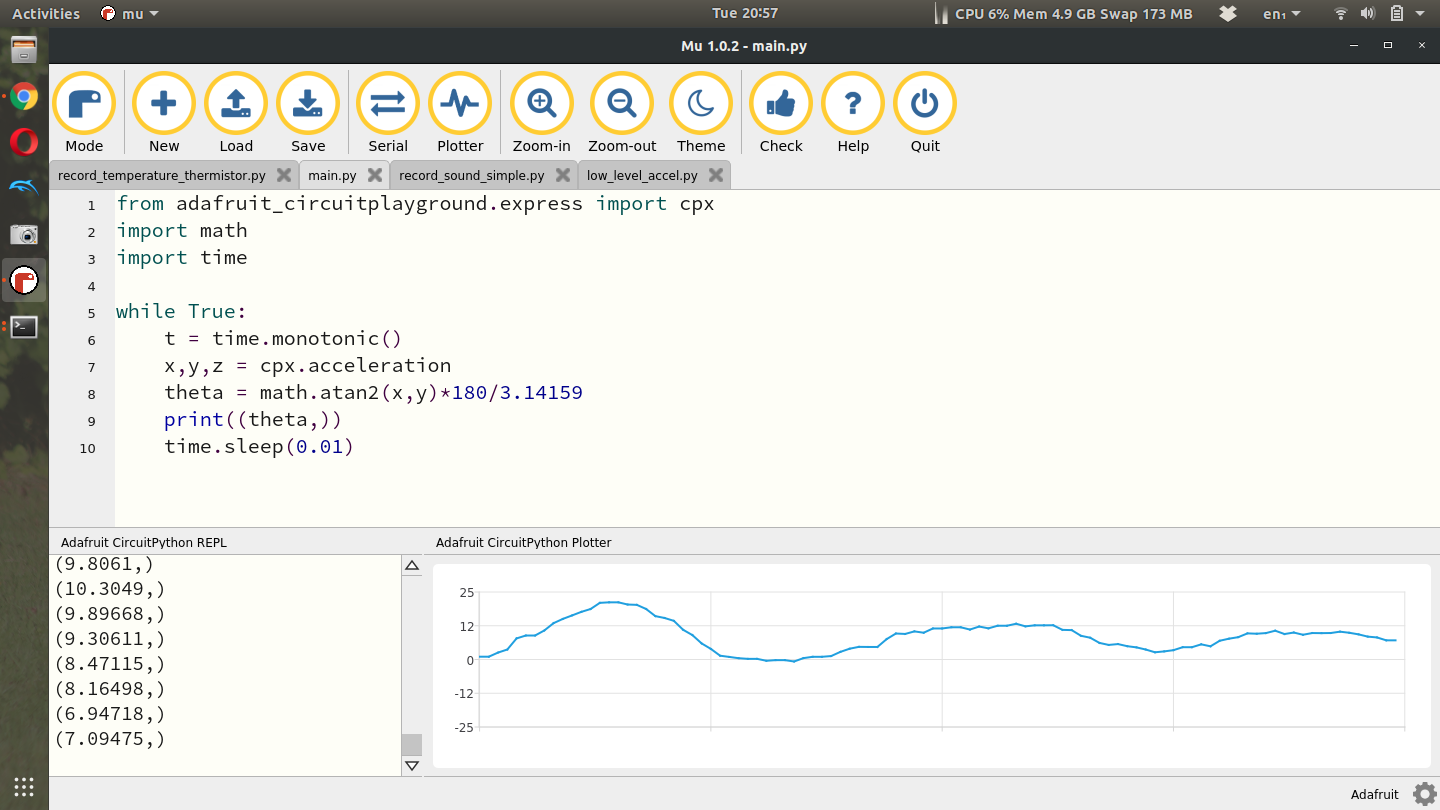
\includegraphics[width=\textwidth]{Figures/oscillation_mu.png}
  \end{center}
\end{figure}

\subsection{Assignment}

Upload a PDF with all of the photos and text below included. My recommendation is for you to create a Word document and insert all the photos and text into the document. Then export the Word document to a PDF. For videos I suggest uploading the videos to Google Drive, turn on link sharing and include a link in your PDF.

\begin{enumerate}[itemsep=-5pt]
\item Include a video of you explaining your experiment. What state are you measuring? What is varying? Show the system varying and explain the code you are using the capture the data. Use the Plotter in Mu to show the system varying. (Make sure you introduce yourself in the video and that you show your face at some point) Explain what you changed about the system to change the natural frequency. I changed the length of my pendulum which changed the natural frequency. What did you change? - 20\%
\item Take data at 3 different frequencies and two different configurations (a total of 6 data sets). Include two plots as I did above with appropriate labels and legends - 20\%
\item Explain the results of your experiment in 1 or 2 paragraphs. Did you encounter any aliasing? Did the amount of aliasing change when you changed the parameters of your system? Why or why not? - 20\%
\item Plot your measured data in Python for your lowest frequency and highest sampling rate and attach a well formatted figure. Include a plot of your fitted data alongside your measured data. Do they match? Why or why not? Write a paragraph explaining your result - 20\%
\item Estimate your damping constant, damped natural frequency, damping ratio, and natural frequency. State these values explicitly in the submission Given the frequency you computed, comment on the frequency you would need to completely avoid aliasing and if the CPX is capable of doing that. - 20\%
\end{enumerate}